
\chapter{Review of Fast Multipole Methods}\label{chpt:fmm}
\thispagestyle{chaptertitle} % Force the fancy style on this page

\begin{center}
    \textit{Portions of the discussion in Sections \ref{chpt:fmm:sec:analytical} and \ref{chpt:fmm:sec:kifmm} of this chapter are adapted from the material first presented in \cite{kailasa2024m2ltranslationoperatorskernel} }
\end{center}

\section{Analytical Fast Multipole Methods}\label{chpt:fmm:sec:analytical}

As in the original presentation, we use the case of evaluating electrostatic potentials to motivate the \acrshort{fmm}. Consider the electric field, $E$ due to a charge distribution $q(\Ybf)$ which is supported over some finite domain $\Ybf \in \Omega \subset \Rd$. It can be defined in terms of a scalar potential $\phi$.

\begin{equation*}
E = -\nabla \phi
\end{equation*}

which itself can be seen to satisfy Poisson's equation,

\begin{equation*}
    \begin{cases}
        - \Delta \phi(\Xbf) = q(\Xbf), \> \> \text{  for } x\in \Rd \\
        \underset{|x| \rightarrow \infty}{\lim } u(\Xbf) = 0
    \end{cases}
\end{equation*}


where $d=2,3$ in problems of interest.

We can write the evaluation of the potential at a point $\Xbf$ as a convolution of the source with the fundamental solution of the Poisson equation,

such that,

\begin{equation}
\phi(\Xbf) = \int_{\Rd} K(\Xbf-\Ybf)q(\Ybf) d\Ybf, \> \> \Xbf \in \Rd
\end{equation}\label{eq:chpt:fmm:laplace_potential_integral}

Under an appropriate discretisation, where care is taken to appropriately handle the singularity in the Laplace kernel (\ref{eq:chpt:introduction:sec:motivation:laplace_kernel}), we see that this integral corresponds to a matrix vector multiplication, where the matrix is \textit{dense}, i.e. it consists of non-zero entries.

As we are principally concerned with the simpler problem of evaluating the potential due to a discrete charge distribution, with $N$ charges we can replace $q(\Ybf)$ with $\{ q(\Ybf_j) \}_{j=1}^N$ associated with \textit{source particles} $\{\Ybf_j\}_{j=1}^N \in \Rd$, the integral for potential evaluated at $M$ \textit{target particles}, $\{\Xbf_i \}_{i=1}^M \in \Rd$ becomes a discrete sum,

\begin{equation}
    \phi(\Xbf_i) = \sum_{j=1}^N K(\Xbf_i-\Ybf_j)q(\Ybf_j), \> \> i = 1,...,M
    \label{eq:chpt:fmm:laplace_potential_sum}
\end{equation}

where we can handle the singularity by setting,

\begin{equation}
    K(\Xbf_i - \Ybf_j) = \begin{cases}
        0, \> \> \Xbf_i = \Ybf_j \\
        K(\Xbf_i - \Ybf_j), \text{  otherwise}
    \end{cases}
\end{equation}


We see that the sum (\ref{eq:chpt:fmm:laplace_potential_sum}) corresponds to a dense matrix vector multiplication,

\begin{equation}
    \phi = K q
\end{equation}


\begin{figure}
    \centering
    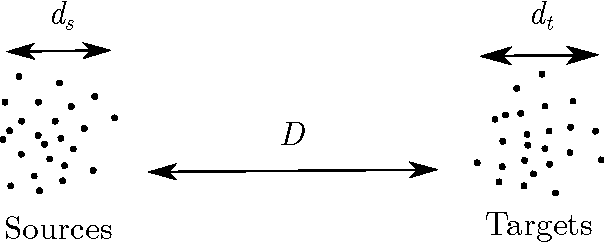
\includegraphics[width=0.5\textwidth]{introduction/degenerate_kernel.pdf}
    \caption{A set of source and target particle cluster, where the width of each cluster is significantly less than the distance separating them, $d_s, d_t \ll D$.}
    \label{fig:chpt:fmm:degenerate_kernel}
\end{figure}

Naively computed this requires $\bigO{MN}$ operations. The \acrshort{fmm} relies on a \textit{degenerate} approximation of the interaction kernel when clusters of source and target particles are sufficiently separated, as sketched in Figure \ref{fig:chpt:fmm:degenerate_kernel}. Following the discussion in \cite{kailasa2024m2ltranslationoperatorskernel} the sum (\ref{eq:chpt:fmm:laplace_potential_sum}) can be written as,

\begin{equation}
    \phi(\Xbf_i) \approx \sum_{p=1}^P \sum_{j=1}^N A_p(\Xbf_i) B_p(\Ybf_j)q(\Ybf_j), \> \> i = 1,...,M
    \label{eq:chpt:introduction:sec:motivation:degenerate_kernel}
\end{equation}

where we call $P$ the expansion order, taken such that $P \ll N$, $P \ll M$. The functions $A_p$ and $B_p$ are defined by the approximation scheme used by a particular approach for the \acrshort{fmm}, in the original presentation the calculation,

\begin{equation}
    \hat{q}_p = \sum_{j=1}^N B_p(\Ybf_j)q(\Ybf_j)
\end{equation}

Corresponded to the coefficients of an order $P$ multipole expansion due to the source charges. Following which the potential is approximated by,

\begin{equation}
    \phi(\Xbf_i) \approx \sum_{p=1}^P A_p(\Xbf_i)\hat{q}_p, \> \> i = 1,...,M
\end{equation}

at the target particles. The approximation of the potential with this scheme can be seen to require $\bigO{P(M+N)}$ operations. The accuracy of this approximation scheme, and the error bounds provided by the \acrshort{fmm}, depends on the distance between the source and target clusters remaining large relative to their width. This condition is often referred to as an \textit{admissibility condition} in the \acrshort{fmm} literature. \acrshort{fmm}s therefore split the sum (\ref{eq:chpt:fmm:laplace_potential_sum}) into \textit{near} and \textit{far} components when considering arbitrary clusters of source and target particles,

\begin{equation}
    \phi(\Xbf_i) = \sum_{\Ybf_j \in \text{Near}(\Xbf_i)} K(\Xbf_i, \Ybf_j) q(\Ybf_j) +  \sum_{\Ybf_j \in \text{Far}(\Xbf_i)} K(\Xbf_i, \Ybf_j) q(\Ybf_j), \> \> i=1,..,M
\end{equation}

In cases where a source and target cluster can be considered \textit{admissable}, i.e. the source cluster is considered in the \textit{far field} of the target cluster such that each $\Ybf_j \in \text{Far}(\Xbf_j)$, we apply the approximation (\ref{eq:chpt:introduction:sec:motivation:degenerate_kernel}). However, when a source and target cluster are \textit{inadmissable}, such that the source cluster is considered in the \textit{near field} of a target cluster such that each $\Ybf_j \in \text{Near}(\Xbf_j)$ we are left to evaluate the sum directly via (\ref{eq:chpt:fmm:laplace_potential_sum}).

In order to achieve its $\bigO{N}$ complexity the FMM is structured to reduce to a minimum the number of sums evaluated between inadmissable clusters. This is achieved with a hierarchical discretisation of the problem domain, often a \textit{quadtree} in two dimensions and correspondingly an \textit{octree} in three dimensions. These data structures are generated by creating a bounding box that covers the source and target particles, which without loss of generality may correspond to the same set. This box is then recursively sub-divided into \textit{child boxes} of equal size.

- Overview of FMM algorithm for non-Oscillatory kernels.

- A brief not on computing changes in the past decades, and which part of the algorithm are a little redundant.

- A reflection on the key hidden constants in complexity, and why this may no longer be the most significant factor in modern implementations.

- A note on FMM software that is available, its positives and negatives, and why this is a little different.

- Conclude with why this thesis exists, to tackle these problems.


\section{Kernel Independent Fast Multipole Methods}\label{chpt:fmm:sec:kifmm}

- Review of the KiFMM and variants. Black Box FMM, Analytical FMM, Data Driven Techniques.

- Motivation for use from a software engineering and computational performance perspective.

- Data flow during the KiFMM.

- Performance characteristics and features of the kiFMM.

- Reflection on the kiFMM and modern software and hardware

The decades since its original presentation have seen the \acrshort{fmm} extended with related ideas which principally differ in how they represent interactions between distant clusters of particles typically referred to as \textit{algebraic} FMMs.


- Black Box vs Analytical

\section{Oscillatory Fast Multipole Methods}

- helmholtz fmm

- high frequency helmholtz FMM, out of scope of the thesis but can mention that they exist. Especially in the context of kiFMM approaches, what is the key difference? When does it apply (the directional low rank condition), where is there an additional loop? Why might this result in greater complexity

\section{Related Ideas}

- H Matrix and H2 matrices, and wider setting of the FMM and related problems.

- Abduljabbar thesis contains a nice summary I can read.


\section{The Fast Multipole Method's Computational Structure}

- Parallelism levels in computing (ILP (Pipelining, Superscalar, Speculative execution), Data level (SIMD, GPU), Thread level TLP (multithreading, simultaneous multithreading and hyper threading), Process level (symettric and asymettrixc multitprocessing), task level, Distributed Parallelism e.g. MPI and MapReduce)

- Only some of these are relevant for scientific computing

- Examine FMM data flow and relate to levels of Parallelism and which will be taken advantage of by us, and which are yet to be examined.

- What is the trend in hardware and why is the FMM a good kernel for scaling in future computer systems?

- What are the principal difficulties we will encounter? Data organisation, and communication costs in a distributed setting.

- What about good FMM software? Specialised kernels and substructures are required to be generically interfaced.

- What parts of this are addressed by this thesis and where?


\section{Review of Software Approaches}

- What software exists, and which approaches do they use?

- What are they optimised for, and what kind of performance do they promise?

- What are the trade-offs of each software

- Hardware targetted by each available software, what's missing?

- What's available, and what are the shortcomings?

- And then

\section{Thesis Structure}\label{chpt:fmm:sec:layout}


In Chapter \ref{chpt:fmm} we perform a literature review of methods and software for modern \acrlong{fmm}s, with a specific focus on so called `kernel independent' or `black box' \acrshort{fmm}s in Sections ... and ... which are the focus of our implementation efforts. We review related ideas which share many features of the \acrshort{kifmm}s in Section ..., such as the $\mathcal{H}$ and $\mathcal{H}^2$ matrix approaches. We move on to a review of the \acrshort{kifmm}s computational structure in Section ..., where we provide estimates of the computational complexities of its operators, and identify the parallelism available in the algorithm with respect to that provided by modern hardware. We conclude with a review of past software efforts for \acrshort{fmm}s, and place our contribution within this context.


A major effort of this thesis was designing a \textit{platform} for \acrshort{kifmm}s. Whereby, one is free to experiment with the implementation of subcomponents in a highly modular way, while retaining performance and the use of the remainder of the library. Therefore a significant early investigation was into appropriate tooling environments for scientific software, first presented in \cite{kailasa2022pyexafmm}. We present this investigation in Chapter \ref{chpt:programming_for_science}, where we document our experience with Python as an alternative for achieving low-level performance as well as our chosen platform Rust, a relatively new language emerging as a contender for performant and productive research software.

Chapter \ref{chpt:field_translation} details a rigorous application of our framework, where we investigated optimisations for the crucial \acrshort{m2l} field translation, recently presented in \cite{kailasa2024m2ltranslationoperatorskernel}. We find non-intuitively that direct matrix compression techniques for admissable blocks can be highly competitive with state of the art optimal schemes based on \acrshort{ffts} for three dimensional problems described by the Laplace kernel.

Chapter \ref{chpt:software_design} describes in detail the engineering approach of our software, particularly the employment of Rust's trait system, as well as specific implementation details of the \acrshort{kifmm}s operators. In Chapter \ref{chpt:hpc} we discuss the design and implementation of our software framework for distributed memory systems, detailing communication reducing schemes for the communication of ghost information.

Chapter \ref{chpt:experiments} contains numerical experiments with our software in a single node (Section ...) as well as HPC (Section ...) setting, including a study of the applicability of our software to problems described by Helmholtz problems with low to moderate wavenumbers.


We conclude with a reflection on our results and suggestions for future investigations in Chapter \ref{chpt:conclusion}.

